% ============================================================
% 第4章：指数函数——增长的终极武器
% ============================================================

\chapter{指数函数——增长的终极武器}

\begin{applicationbox}
\textbf{学完本章你能做什么？}
\begin{enumerate}
  \item \textbf{学之前}：你知道 \(x^2\)、\(x^3\) 这种幂函数，但它们的增长受限于指数大小。
  \item \textbf{学之后}：你会看到指数函数 \(2^x\) 最终会\textbf{超过任何幂函数}——这就是指数增长的威力。
        你还会理解 AI 中 Softmax 和 Sigmoid 为什么离不开指数。
  \item \textbf{日常例子}：一张纸对折 50 次后有多厚？
        每次对折厚度翻倍——\(2^{50}\) 张纸的厚度 ≈ 1亿公里，超过地球到太阳的距离！
        这就是指数增长。
\end{enumerate}
\end{applicationbox}


% ============================================================
\section{从第3章来——幂函数 vs 指数函数}
% ============================================================

第3章我们学了幂函数 \(y = x^n\)——底是变量 \(x\)，指数是常数 \(n\)。

现在反过来：\textbf{底是常数，指数是变量}——这就是\textbf{指数函数}。

\begin{center}
\begin{tabular}{c|c|c}
 & \textbf{幂函数} & \textbf{指数函数} \\
\hline
形式 & \(y = x^n\) & \(y = a^x\) \\
例子 & \(y = x^2\)（底变、指数不变） & \(y = 2^x\)（指数变、底不变） \\
增长特点 & 多项式增长 & \textbf{指数增长（碾压级）} \\
\end{tabular}
\end{center}


% ============================================================
\section{指数函数的定义}
% ============================================================

\begin{definitionbox}[指数函数]
形如
\[
f(x) = a^x \quad (a > 0,\; a \neq 1)
\]
的函数称为\textbf{指数函数}（读作 zhǐ shù hán shù，英文 exponential function），
其中 \(a\) 是\textbf{底数}，\(x\) 是\textbf{自变量}（指数）。

\textbf{为什么 \(a > 0\) 且 \(a \neq 1\)？}
\begin{itemize}
  \item \(a > 0\)：负数底数的分数次方可能无意义（如 \((-2)^{1/2} = \sqrt{-2}\)）
  \item \(a \neq 1\)：\(1^x = 1\) 是常数，没意思
\end{itemize}
\end{definitionbox}

\begin{examplebox}[1——指数函数 vs 幂函数]
判断下列函数是指数函数还是幂函数：
\begin{align*}
  &f(x) = 3^x \quad &\text{指数函数（底固定 3，指数变）} \\
  &g(x) = x^3 \quad &\text{幂函数（底变，指数固定 3）} \\
  &h(x) = 2^{x} + 1 \quad &\text{指数函数+常数} \\
  &p(x) = x^{\pi} \quad &\text{幂函数（指数是常数 \(\pi\)）}
\end{align*}

\textbf{快速判断法：}变量在指数上 \(\rightarrow\) 指数函数；变量在底上 \(\rightarrow\) 幂函数。
\end{examplebox}


% ============================================================
\section{底 > 1：指数增长}
% ============================================================

当底数 \(a > 1\) 时，函数值随着 \(x\) 增大而\textbf{快速增长}。

\begin{examplebox}[2]
对比 \(y = 2^x\)、\(y = 3^x\)、\(y = 5^x\)、\(y = 10^x\)：

\begin{center}
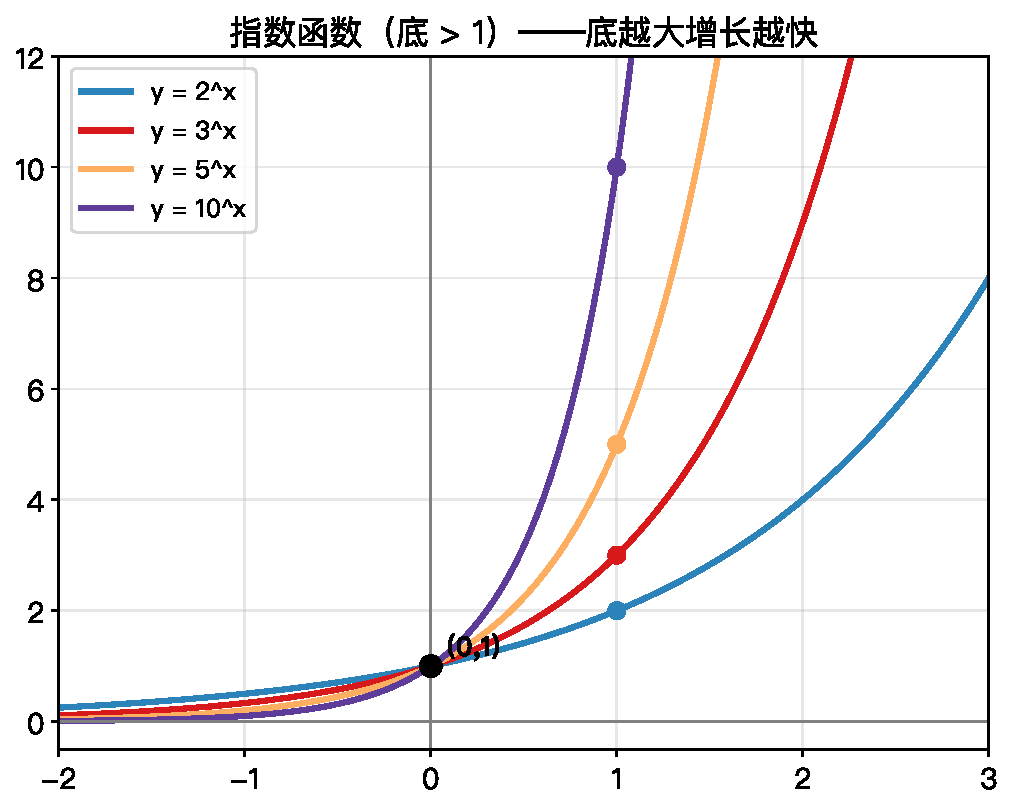
\includegraphics[width=0.6\textwidth]{figures/ch04_exponential_growth.pdf}
\end{center}

\textbf{观察规律：}
\begin{enumerate}
  \item 所有图像都经过 \((0,1)\)——因为 \(a^0 = 1\)
  \item 所有图像都经过 \((1,a)\)——因为 \(a^1 = a\)
  \item 底越大，增长越快（\(10^x\) 比 \(2^x\) 陡得多）
  \item 当 \(x < 0\) 时，函数值在 0 和 1 之间（如 \(2^{-1} = 0.5\)）
  \item 图像始终在 \(x\) 轴上方（\(a^x > 0\) 对所有实数 \(x\) 成立）
\end{enumerate}
\end{examplebox}

\begin{definitionbox}[指数函数的性质（底 > 1）]
\[
f(x) = a^x,\; a > 1
\]
\begin{itemize}
  \item \textbf{定义域}：\(\mathbb{R}\)（全体实数）
  \item \textbf{值域}：\((0, +\infty)\)（永远为正，但可以无限接近 0）
  \item \textbf{单调性}：严格递增（\(x_1 < x_2 \Rightarrow a^{x_1} < a^{x_2}\)）
  \item \textbf{水平渐近线}：\(y = 0\)（当 \(x \to -\infty\) 时，\(a^x \to 0\)）
  \item \textbf{经过点}：\((0,1)\)、\((1,a)\)
\end{itemize}
\end{definitionbox}


% ============================================================
\section{0 < 底 < 1：指数衰减}
% ============================================================

当底数在 0 和 1 之间时，函数值随着 \(x\) 增大而\textbf{逐渐衰减}。

\begin{examplebox}[3]
对比 \(y = (1/2)^x\)、\(y = (1/3)^x\)、\(y = (1/5)^x\)：

\begin{center}
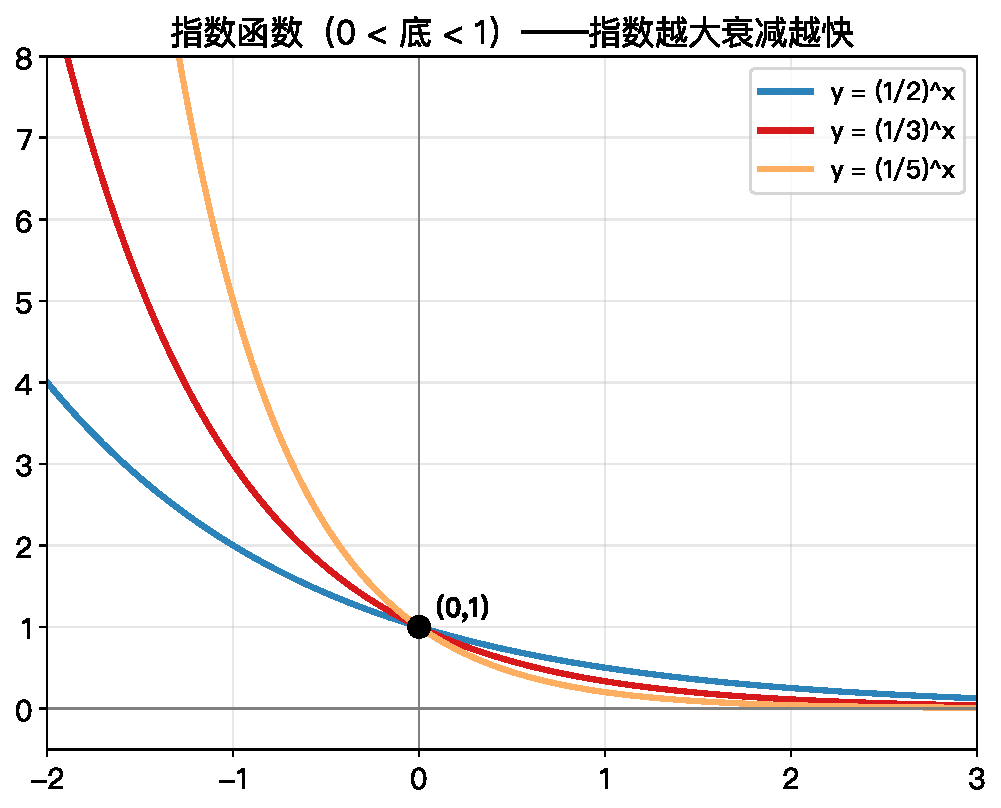
\includegraphics[width=0.6\textwidth]{figures/ch04_exponential_decay.pdf}
\end{center}

\textbf{观察规律：}
\begin{enumerate}
  \item 同样经过 \((0,1)\)
  \item 但这次是\textbf{递减}的——\(x\) 越大，函数值越小
  \item 底越小，衰减越快（\((1/5)^x\) 比 \((1/2)^x\) 下降得更快）
  \item 当 \(x \to +\infty\) 时，函数值趋近于 0
  \item 水平渐近线仍然是 \(y = 0\)
\end{enumerate}
\end{examplebox}


% ============================================================
\section{增长与衰减的对称关系}
% ============================================================

增长型 \(y = a^x\) 和衰减型 \(y = (1/a)^x\) 之间有优美的对称关系。

\begin{examplebox}[4]
\(y = 2^x\) 和 \(y = (1/2)^x\) 关于 \(y\) 轴对称：

\begin{center}
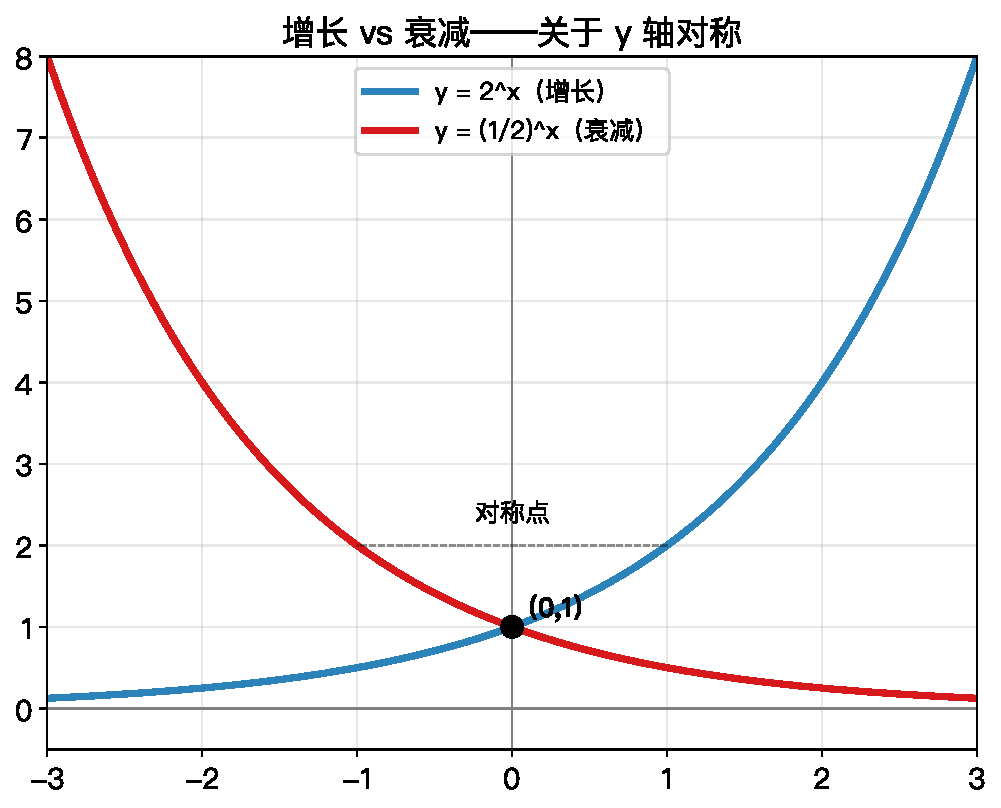
\includegraphics[width=0.6\textwidth]{figures/ch04_growth_vs_decay.pdf}
\end{center}

\textbf{原因：}
\[
\left(\frac{1}{2}\right)^x = (2^{-1})^x = 2^{-x}
\]

所以 \(y = (1/2)^x\) 其实就是 \(y = 2^{-x}\)——把 \(x\) 换成 \(-x\)，图像关于 \(y\) 轴对称。

\textbf{一般规律：}
\[
\boxed{a^x \text{ 和 } (1/a)^x \text{ 关于 } y \text{ 轴对称}}
\]
\end{examplebox}


% ============================================================
\section{自然指数 \(e^x\)——最重要的指数函数}
% ============================================================

在所有可能的底数中，有一个底数\textbf{特别重要}——它就是 \(e\)。

\begin{definitionbox}[自然常数 \(e\)]
\(e\) 是一个无理数，约等于 2.71828\ldots

它是自然对数的底数，也是数学中最重要的常数之一（和 \(\pi\) 齐名）。
\end{definitionbox}

\begin{examplebox}[5]
\(y = e^x\) 与 \(2^x\)、\(3^x\) 的对比：

\begin{center}
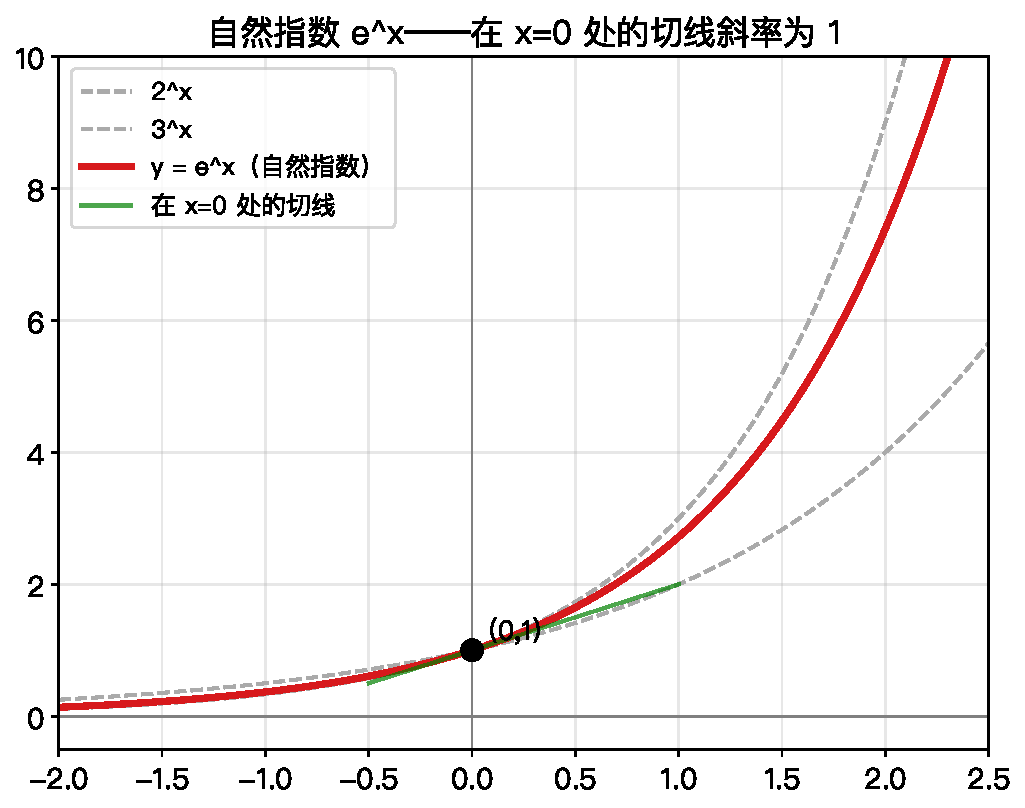
\includegraphics[width=0.6\textwidth]{figures/ch04_natural_exponential.pdf}
\end{center}

\textbf{为什么 \(e^x\) 这么重要？}
\begin{enumerate}
  \item 在 \(x=0\) 处，\(e^x\) 的切线斜率为 1（精确等于 1！）
  \item 这一点使得 \(e^x\) 的导数就是它自己（以后学导数时会详细讲）
  \item 自然界的很多现象都用 \(e^x\) 描述：人口增长、放射性衰变、复利计算
  \item AI 中 Softmax 的核心就是 \(e^x\)
\end{enumerate}
\end{examplebox}


% ============================================================
\section{指数函数 vs 幂函数——谁增长更快？}
% ============================================================

这是数学中一个\textbf{非常重要的结论}：

\begin{center}
\fcolorbox{red!50}{red!5}{\parbox{0.85\textwidth}{
\textbf{指数增长最终会超过任何幂函数增长。}\\
不管幂函数的指数多大（即使是 \(x^{100}\)），
总存在某个点之后，\textbf{指数函数永远大于幂函数}。
}}
\end{center}

\begin{examplebox}[6]
对比 \(2^x\)、\(x^2\)、\(x^3\)：

\begin{center}
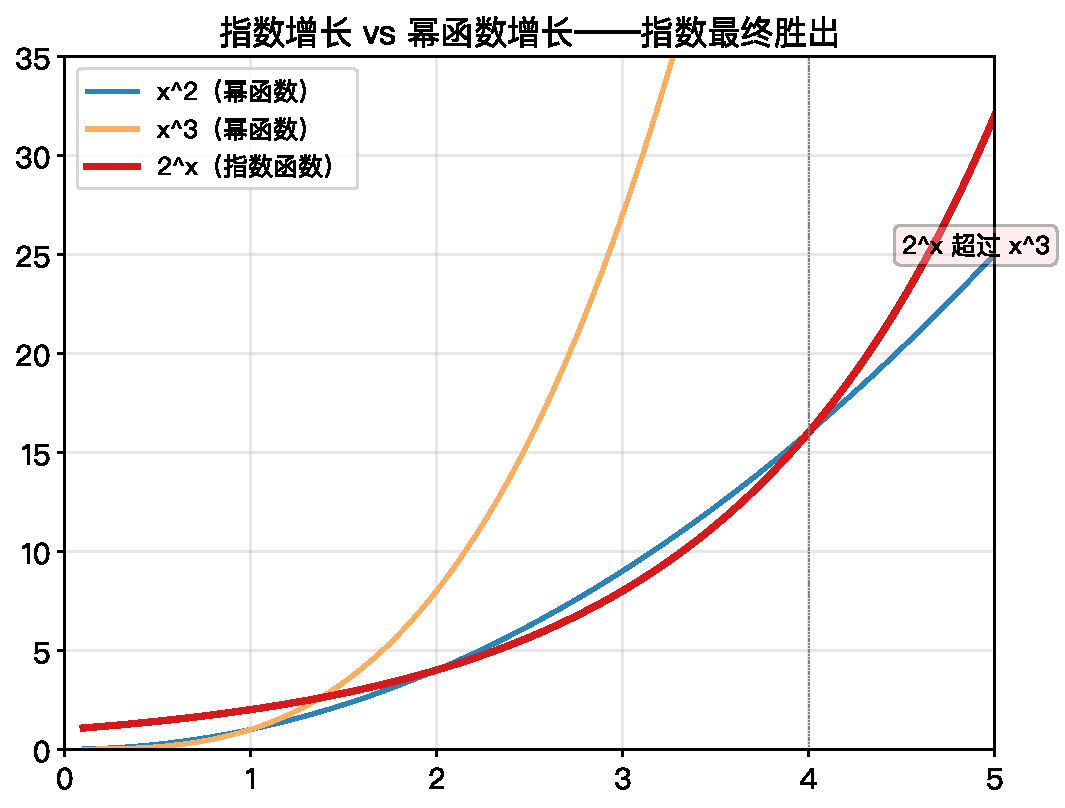
\includegraphics[width=0.6\textwidth]{figures/ch04_expo_vs_power.pdf}
\end{center}

\textbf{验证：}
\begin{center}
\begin{tabular}{c|c|c|c}
\(x\) & \(x^2\) & \(x^3\) & \(2^x\) \\
\hline
0 & 0 & 0 & 1 \\
1 & 1 & 1 & 2 \\
2 & 4 & 8 & 4 \\
3 & 9 & 27 & 8 \\
4 & 16 & 64 & 16 \\
5 & 25 & 125 & 32 \\
6 & 36 & 216 & 64 \\
7 & 49 & 343 & 128 \\
8 & 64 & 512 & 256 \\
9 & 81 & 729 & 512 \\
10 & 100 & 1000 & 1024 \\
\end{tabular}
\end{center}

在 \(x = 10\) 时，\(2^x = 1024\) 已经超过了 \(x^3 = 1000\)。
虽然 \(x^3\) 一开始领先，但指数函数\textbf{终究会超越}。
\end{examplebox}


% ============================================================
\section{指数方程}
% ============================================================

\begin{definitionbox}[指数方程]
指数里含有未知数的方程叫\textbf{指数方程}。

基本解法：将两边化为\textbf{同底}形式，然后让指数相等。
\[
a^{f(x)} = a^{g(x)} \quad\Longrightarrow\quad f(x) = g(x)
\]
\end{definitionbox}

\begin{examplebox}[7——解指数方程]
解方程：
\[
(1)\; 2^x = 8 \qquad (2)\; 3^{x+1} = 27 \qquad (3)\; 2^{2x-1} = 4^{x+3}
\]

解：
\[
\begin{aligned}
(1)&\; 2^x = 8 = 2^3 \;\Longrightarrow\; x = 3 \\
(2)&\; 3^{x+1} = 27 = 3^3 \;\Longrightarrow\; x+1 = 3 \;\Longrightarrow\; x = 2 \\
(3)&\; 2^{2x-1} = 4^{x+3} = (2^2)^{x+3} = 2^{2x+6} \\
    &\;\Longrightarrow\; 2x-1 = 2x+6 \;\Longrightarrow\; -1 = 6 \;\Longrightarrow\; \text{无解}
\end{aligned}
\]

\textbf{注意：} 第(3)题无解的原因是左右两边不可能相等。\\
\textbf{验证：} 左边 \(2^{2x-1}\)，右边 \(4^{x+3} = 2^{2x+6}\)，右边总是比左边大 \(2^7 = 128\) 倍。
\end{examplebox}

\begin{examplebox}[8——指数不等式]
解不等式 \(2^x > 8\)：

\[
2^x > 8 = 2^3 \;\Longrightarrow\; x > 3
\]

因为底数 \(2 > 1\)，指数函数递增，所以不等号方向不变。

如果底数在 0 和 1 之间，不等号会反向：
\[
\left(\frac{1}{2}\right)^x > \frac{1}{8} \;\Longrightarrow\; \left(\frac{1}{2}\right)^x > \left(\frac{1}{2}\right)^3 \;\Longrightarrow\; x < 3
\]
\end{examplebox}


% ============================================================
\section{指数函数在 AI 中的应用}
% ============================================================

\begin{examplebox}[9——Softmax 函数]
Softmax 是 AI 中最常用的函数之一，它将一组数转换成"概率"。

\[
\text{Softmax}(x_i) = \frac{e^{x_i}}{\sum_{j} e^{x_j}}
\]

\textbf{为什么用指数？}
\begin{enumerate}
  \item 指数保证输出为正数（概率不能为负）
  \item 指数放大了差距——输入的微小差异在输出中会被放大
  \item 所有输出的和为 1（满足概率的定义）
\end{enumerate}

\textbf{例：} 输入 \([2, 1, 0]\)：
\[
e^2 \approx 7.39,\quad e^1 \approx 2.72,\quad e^0 = 1
\]
\[
\text{Softmax} = \left[\frac{7.39}{7.39+2.72+1},\; \frac{2.72}{11.11},\; \frac{1}{11.11}\right] \approx [0.67, 0.24, 0.09]
\]

最大输入 2 被放大成了概率 67\%，这就是 Softmax 的"赢家通吃"效果。
\end{examplebox}


% ============================================================
\section{符号卡片}
% ============================================================

\begin{symbolcard}
\(a^x\) & \verb|a^x| & 读作"a 的 x 次方" & 指数函数，底 \(a\) 指数 \(x\) \\
\(e\) & \verb|e| & 读作"自然常数" & 约 2.71828，最重要的底数 \\
\(e^x\) & \verb|e^x| & 读作"e 的 x 次方" & 自然指数函数 \\
\((0, +\infty)\) & \verb|(0, +inf)| & 读作"0 到正无穷" & 指数函数的值域 \\
水平渐近线 & —— & —— & 指数函数当 \(x\to -\infty\) 时的极限 \\
\end{symbolcard}


% ============================================================
\section{代码验证}
% ============================================================

\begin{lstlisting}[caption=指数函数的数值验证]
import numpy as np

# 1. 验证指数函数经过 (0,1) 和 (1,a)
print("=== 指数函数经过 (0,1) ===")
for a in [2, 3, 5, 10]:
    print(f"  {a}^0 = {a**0},  {a}^1 = {a**1}")
print(f"  e^0 = {np.e**0},  e^1 = {np.e**1:.4f}")

print()

# 2. 指数增长 vs 幂函数增长
print("=== 指数 vs 幂函数（看谁大）===")
for x in range(0, 11):
    power2 = x**2
    power3 = x**3
    expo = 2**x
    winner = "指数!" if expo > power3 else ("幂函数" if power3 > expo else "打平")
    print(f"  x={x:2d}:  x^2={power2:4d},  x^3={power3:4d},  2^x={expo:5d}  <- {winner}")

print()

# 3. Softmax 模拟
def softmax(x):
    e_x = np.exp(x - np.max(x))  # 稳定版
    return e_x / np.sum(e_x)

scores = np.array([2.0, 1.0, 0.0])
probs = softmax(scores)
print("=== Softmax 示例 ===")
for i, (s, p) in enumerate(zip(scores, probs)):
    print(f"  输入 {s:.1f} -> 概率 {p:.3f} ({p*100:.1f}%)")
print(f"  概率和 = {np.sum(probs):.6f}")
\end{lstlisting}

运行结果：
\begin{lstlisting}[frame=none,backgroundcolor={},numbers=none]
=== 指数函数经过 (0,1) ===
  2^0 = 1,  2^1 = 2
  3^0 = 1,  3^1 = 3
  5^0 = 1,  5^1 = 5
  10^0 = 1,  10^1 = 10
  e^0 = 1,  e^1 = 2.7183

=== 指数 vs 幂函数（看谁大）===
  x= 0:  x^2=   0,  x^3=   0,  2^x=    1  <- 指数!
  x= 1:  x^2=   1,  x^3=   1,  2^x=    2  <- 指数!
  x= 2:  x^2=   4,  x^3=   8,  2^x=    4  <- 幂函数
  x= 3:  x^2=   9,  x^3=  27,  2^x=    8  <- 幂函数
  x= 4:  x^2=  16,  x^3=  64,  2^x=   16  <- 幂函数
  x= 5:  x^2=  25,  x^3= 125,  2^x=   32  <- 幂函数
  x= 6:  x^2=  36,  x^3= 216,  2^x=   64  <- 幂函数
  x= 7:  x^2=  49,  x^3= 343,  2^x=  128  <- 幂函数
  x= 8:  x^2=  64,  x^3= 512,  2^x=  256  <- 幂函数
  x= 9:  x^2=  81,  x^3= 729,  2^x=  512  <- 幂函数
  x=10:  x^2= 100,  x^3=1000,  2^x= 1024  <- 指数!

=== Softmax 示例 ===
  输入 2.0 -> 概率 0.665 (66.5%)
  输入 1.0 -> 概率 0.245 (24.5%)
  输入 0.0 -> 概率 0.090 (9.0%)
  概率和 = 1.000000
\end{lstlisting}


% ============================================================
\section{本章小结}
% ============================================================

\begin{progressbox}
\textbf{指数函数} \(y = a^x\)：底固定、指数变。所有指数函数经过 \((0,1)\) 和 \((1,a)\)。

\textbf{底 > 1}（增长型）：递增，底越大增长越快
\textbf{0 < 底 < 1}（衰减型）：递减，底越小衰减越快

\textbf{对称性}：\(a^x\) 和 \((1/a)^x\) 关于 \(y\) 轴对称

\textbf{自然指数} \(e^x\)：在 \(x=0\) 处切线斜率为 1，导数等于自己

\textbf{指数 vs 幂函数}：指数函数\textbf{最终胜出}——这是数学中最重要的增长对比

\textbf{AI 应用}：Softmax 用指数把输入转换成概率，放大差距
\end{progressbox}

\subsection*{通往下一章}

\textbf{这一章}你学会了指数函数——增长的终极武器。

\textbf{下一章}我们学\textbf{对数函数}——指数的"逆运算"。
如果说指数回答的是"给定底数和指数，结果是多少"，对数回答的就是\,"给定底数和结果，指数是多少"。
这两个函数是数学中最重要的"搭档"。


% ============================================================
% 习题
% ============================================================
\section{习题}

% ===== 送分 =====

\begin{exercise}[0]
判断是指数函数还是幂函数：
\[
(1)\; y = 4^x \quad (2)\; y = x^4 \quad (3)\; y = \pi^x \quad (4)\; y = x^{\pi}
\]
\GoodExercise{exp-vs-power}
\end{exercise}

\begin{exercise}[0]
计算：
\[
(1)\; 2^3 \quad (2)\; 2^0 \quad (3)\; 2^{-2} \quad (4)\; 4^{1/2}
\]
\end{exercise}

\begin{exercise}[0]
指数函数 \(y = 3^x\) 经过哪两个固定点？
\end{exercise}

\begin{exercise}[0]
比较大小（不用计算器）：
\[
(1)\; 2^3 \text{ 和 } 3^2 \qquad
(2)\; 2^{-1} \text{ 和 } 2^0
\]
\end{exercise}

% ===== 简单 =====

\begin{exercise}[1]
画出 \(y = 2^x\) 的草图（取 \(x = -2, -1, 0, 1, 2\) 五个点），标出关键点坐标。
\end{exercise}

\begin{exercise}[1]
判断 \(y = 3^x\) 是递增还是递减？\(y = (1/3)^x\) 呢？
\end{exercise}

\begin{exercise}[1]
计算：
\[
(1)\; 2^3 \times 2^4 \qquad (2)\; \frac{3^5}{3^2} \qquad (3)\; (2^2)^3
\]
\end{exercise}

\begin{exercise}[1]
填空：当 \(x\) 很大时，\(2^x\) 的值趋近于\_\_\_\_；当 \(x\) 很负时，\(2^x\) 的值趋近于\_\_\_\_。
\end{exercise}

% ===== 基础 =====

\begin{exercise}[2]
在同一坐标系中画出 \(y = 2^x\) 和 \(y = (1/2)^x\) 的草图，它们是什么关系？
\end{exercise}

\begin{exercise}[2]
解方程：
\[
(1)\; 2^x = 16 \qquad (2)\; 3^{x-1} = 27 \qquad (3)\; 5^{2x} = 25
\]
\end{exercise}

\begin{exercise}[2]
比较大小：
\[
(1)\; 2^{0.5} \text{ 和 } 2^{0.8} \qquad
(2)\; (0.5)^{0.5} \text{ 和 } (0.5)^{0.8} \qquad
\]
（提示：注意底数是否大于 1）
\end{exercise}

\begin{exercise}[2]
一种细菌每 30 分钟分裂一次（数量翻倍）。开始时只有 1 个细菌，\(t\) 小时后有多少个？
写出表达式。
\end{exercise}

% ===== 普通 =====

\begin{exercise}[3]
已知 \(f(x) = 2^x\)，求：
\[
f(0),\; f(1),\; f(-2),\; f(a),\; f(a+1)
\]
\end{exercise}

\begin{exercise}[3]
解不等式：
\[
(1)\; 2^x > 32 \qquad (2)\; 3^{x-1} \le 9 \qquad (3)\; (1/2)^x > 1/8
\]
\end{exercise}

\begin{exercise}[3]
\(y = 2^x + 1\) 的图像是由 \(y = 2^x\) 经过什么变换得到的？它的水平渐近线是什么？
\end{exercise}

\begin{exercise}[3]
比较 \(2^x\) 和 \(x^2\) 的大小关系（取 \(x = 1, 2, 3, 4, 5\) 分别计算并比较）。
\end{exercise}

\begin{exercise}[3]
某种放射性物质每年衰减 5\%（即每年剩余为上一年的 95\%）。初始质量为 100 克。
\begin{enumerate}
  \item[(1)] 写出 \(t\) 年后的质量表达式
  \item[(2)] 求 10 年后的剩余质量（保留整数）
\end{enumerate}
\end{exercise}

% ===== 中等 =====

\begin{exercise}[4]
解方程：
\[
(1)\; 2^{x+1} = 4^{x-1} \qquad (2)\; 3^{2x} - 3^x - 6 = 0
\]
（提示：(2) 令 \(t = 3^x\)，化为关于 \(t\) 的二次方程）
\end{exercise}

\begin{exercise}[4]
已知 \(f(x) = a^x\) 经过点 \((2, 9)\)，求 \(a\) 的值，并写出 \(f(x)\) 的表达式。
\end{exercise}

\begin{exercise}[4]
\(y = 3^{x-2} + 1\) 是由 \(y = 3^x\) 经过怎样的平移得到的？
它的值域和水平渐近线是什么？
\end{exercise}

\begin{exercise}[4]
某城市人口每年增长 2\%。现在有 100 万人，多少年后人口翻倍？
（提示：解 \(100 \times 1.02^t = 200\)，尝试 \(t = 35\) 和 \(t = 36\) 看看哪个接近）
\end{exercise}

\begin{exercise}[4]
对于 \(y = a^x\)（\(a > 0, a \neq 1\)），证明：
\[
f(x) \cdot f(y) = f(x + y)
\]
并用这个性质计算 \(2^3 \times 2^4\)。
\end{exercise}

% ===== 进阶 =====

\begin{exercise}[5]
解方程 \(4^x - 2^{x+1} - 8 = 0\)。
（提示：\(4^x = (2^2)^x = 2^{2x} = (2^x)^2\)，令 \(t = 2^x\)）
\end{exercise}

\begin{exercise}[5]
已知函数 \(f(x) = 2^x - 2^{-x}\)。
\begin{enumerate}
  \item[(1)] 判断 \(f(x)\) 的奇偶性
  \item[(2)] 证明 \(f(x)\) 是递增函数
\end{enumerate}
\end{exercise}

\begin{exercise}[5]
某种药物的血药浓度随时间变化为 \(C(t) = C_0 \cdot e^{-kt}\)。
已知初始浓度 \(C_0 = 100\)，2 小时后浓度降为 50。
\begin{enumerate}
  \item[(1)] 求 \(k\) 的值
  \item[(2)] 4 小时后的浓度是多少？
\end{enumerate}
\end{exercise}

\begin{exercise}[5]
比较 \(2^{\pi}\) 和 \(\pi^2\) 的大小（提示：\(2^\pi\) 是指数，\(\pi^2\) 是幂函数）。
\end{exercise}

% ===== 拔高 =====

\begin{exercise}[6]
已知 \(f(x) = \dfrac{e^x - e^{-x}}{2}\)（这个函数叫双曲正弦，以后会学到）。
\begin{enumerate}
  \item[(1)] 证明 \(f\) 是奇函数
  \item[(2)] 证明 \(f\) 是递增函数
  \item[(3)] 解方程 \(f(x) = 1\)（提示：令 \(t = e^x\)）
\end{enumerate}
\end{exercise}

\begin{exercise}[6]
对于指数函数 \(f(x) = a^x\)（\(a > 1\)），证明：
\[
\frac{f(x_1) + f(x_2)}{2} \ge f\left(\frac{x_1 + x_2}{2}\right)
\]
这个性质叫\textbf{指数函数的凸性}——图像始终在弦的下方（以后学导数时会用这个性质）。
\end{exercise}

\begin{exercise}[6]
已知 \(a > 0, a \neq 1\)，\(f(x) = a^{x} + a^{-x}\)。
\begin{enumerate}
  \item[(1)] 判断奇偶性
  \item[(2)] 求最小值（提示：利用 \(a^x + a^{-x} \ge 2\) 的基本不等式）
\end{enumerate}
\end{exercise}

% ===== 极难 =====

\begin{exercise}[7]
已知 \(f(x) = 2^x\)，\(g(x) = x^2\)。
\begin{enumerate}
  \item[(1)] 列出 \(x = 1, 2, 3, 4, 5, 10, 20\) 时 \(f(x)\) 和 \(g(x)\) 的值
  \item[(2)] 证明：存在一个 \(N\)，使得对所有 \(x > N\)，有 \(2^x > x^2\)
  \item[(3)] 找到最小的整数 \(N\) 满足这个性质
\end{enumerate}

\textbf{说明：} 这道题让你亲手验证"指数函数最终超过幂函数"这个重要结论。
找到那个"转折点"N 是数学分析中常见的思维方式。
\end{exercise}
